\documentclass[tikz,border=10pt]{standalone}
\usepackage{tikz}
\usetikzlibrary{arrows.meta,positioning,calc,backgrounds,fit,shapes.geometric}
\usepackage[scaled=0.92]{helvet}
\renewcommand{\familydefault}{\sfdefault}
\usepackage{amsmath,amssymb}
\definecolor{ink}{HTML}{262624}
\definecolor{mute}{HTML}{8A8984}
\definecolor{line}{HTML}{BDBBB5}
\definecolor{acc}{HTML}{2A78D6}
\definecolor{accbg}{HTML}{F1F6FD}
\tikzset{
  >={Latex[length=2.2mm]},
  every node/.style={text=ink},
  b/.style={draw=line, fill=white, rounded corners=2pt, align=center, inner sep=6pt,
            minimum height=10mm, text width=#1, font=\small},
  b/.default=40mm,
  a/.style={b=#1, draw=acc, fill=accbg},
  a/.default=40mm,
  t/.style={font=\footnotesize, text=mute, align=center},
  e/.style={->, draw=mute, line width=0.6pt},
  ea/.style={->, draw=acc, line width=0.9pt},
  eh/.style={->, draw=acc, line width=0.9pt, dash pattern=on 3pt off 2pt},
}

\begin{document}
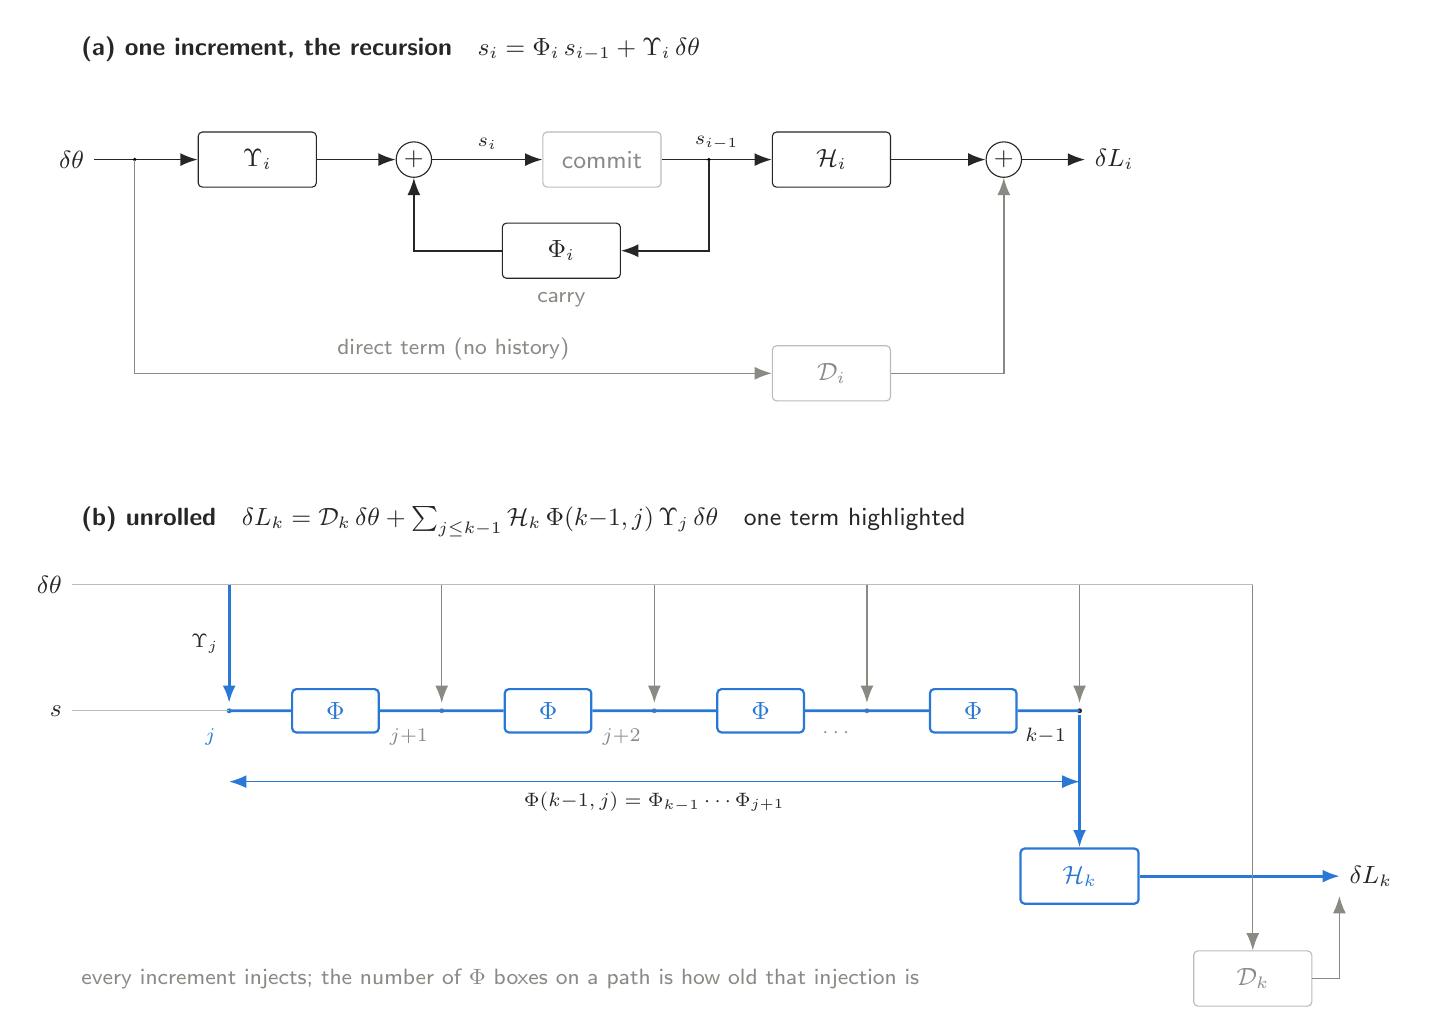
\begin{tikzpicture}
\tikzset{
  op/.style={draw=ink, fill=white, rounded corners=1.5pt, minimum width=15mm, minimum height=7mm, font=\small},
  opg/.style={op, draw=line, text=mute},
  opb/.style={op, draw=acc, text=acc, line width=0.8pt},
  sum/.style={circle, draw=ink, fill=white, inner sep=0pt, minimum size=4.5mm, font=\small},
  w/.style={->, draw=ink, line width=0.6pt},
  wg/.style={->, draw=mute, line width=0.5pt},
  wb/.style={->, draw=acc, line width=1pt},
}
% ------------------- (a) one increment -------------------
\node[anchor=west, font=\small] at (0,0) {\textbf{(a) one increment, the recursion}\quad $s_i = \Phi_i\, s_{i-1} + \Upsilon_i\,\delta\theta$};
\node[font=\small] (in) at (0,-14mm) {$\delta\theta$};
\coordinate (j) at (8mm,-14mm);
\node[op, right=8mm of j] (U) {$\Upsilon_i$};
\node[sum, right=10mm of U] (s1) {$+$};
\node[opg, right=14mm of s1] (cm) {commit};
\coordinate[right=6mm of cm] (j2);
\node[op, right=8mm of j2] (H) {$\mathcal H_i$};
\node[sum, right=12mm of H] (s2) {$+$};
\node[font=\small, right=8mm of s2] (out) {$\delta L_i$};
\node[op, below=8mm of $(s1)!0.5!(j2)$] (P) {$\Phi_i$};
\node[opg, below=20mm of H] (D) {$\mathcal D_i$};
\draw[w] (in) -- (U); \fill (j) circle (0.7pt);
\draw[w] (U) -- (s1); \draw[w] (s1) -- node[above, font=\scriptsize]{$s_i$} (cm);
\draw[w] (cm) -- node[above, font=\scriptsize]{$s_{i-1}$} (H); \fill (j2) circle (0.7pt);
\draw[w] (H) -- (s2); \draw[w] (s2) -- (out);
\draw[w] (j2) |- (P); \draw[w] (P) -| (s1);
\node[t, below=0.5mm of P] {carry};
\draw[wg] (j) |- (D); \draw[wg] (D) -| (s2);
\node[t, anchor=south] at ($(j |- D)!0.5!(D.west)+(0,0.5mm)$) {direct term (no history)};
% ------------------- (b) unrolled -------------------
\begin{scope}[shift={(0,-60mm)}]
\node[anchor=west, font=\small] at (0,0) {\textbf{(b) unrolled}\quad $\delta L_k = \mathcal D_k\,\delta\theta + \sum_{j\le k-1}\mathcal H_k\,\Phi(k{-}1,j)\,\Upsilon_j\,\delta\theta$\quad one term highlighted};
\draw[line, line width=0.5pt] (0,-8mm) -- (150mm,-8mm);
\node[font=\small, anchor=east] at (0,-8mm) {$\delta\theta$};
\node[font=\small, anchor=east] at (0,-24mm) {$s$};
\foreach \x/\lab/\c in {20/j/acc, 47/j{+}1/mute, 74/j{+}2/mute, 101/\cdots/mute, 128/k{-}1/ink} {
  \fill[\c] (\x mm,-24mm) circle (0.9pt);
  \node[font=\scriptsize, text=\c, below left=1mm and 0.5mm] at (\x mm,-24mm) {$\lab$};
}
\draw[wb] (20mm,-8mm) -- node[left, font=\scriptsize]{$\Upsilon_j$} (20mm,-23mm);
\foreach \x in {47,74,101,128} \draw[wg] (\x mm,-8mm) -- (\x mm,-23mm);
\draw[line, line width=0.5pt] (0,-24mm) -- (20mm,-24mm);
\foreach \a/\b in {20/47,47/74,74/101,101/128} {
  \node[opb, minimum width=11mm, minimum height=5.5mm] (p\a) at ($(\a mm,-24mm)!0.5!(\b mm,-24mm)$) {$\Phi$};
  \draw[acc, line width=1pt] (\a mm,-24mm) -- (p\a.west); \draw[acc, line width=1pt] (p\a.east) -- (\b mm,-24mm);
}
\draw[<->, acc, line width=0.5pt] (20mm,-33mm) -- node[below, font=\scriptsize]{$\Phi(k{-}1,j) = \Phi_{k-1}\cdots\Phi_{j+1}$} (128mm,-33mm);
\node[opb] (Hk) at (128mm,-45mm) {$\mathcal H_k$};
\draw[wb] (128mm,-24.5mm) -- (Hk);
\node[font=\small] (Lk) at (165mm,-45mm) {$\delta L_k$};
\draw[wb] (Hk) -- (Lk);
\node[opg] (Dk) at (150mm,-58mm) {$\mathcal D_k$};
\draw[wg] (150mm,-8mm) -- (Dk); \draw[wg] (Dk) -| ($(Lk.south)+(-4mm,0)$);
\node[t, anchor=west, align=left] at (0,-58mm) {every increment injects; the number of $\Phi$ boxes on a path is how old that injection is};
\end{scope}
\end{tikzpicture}
\end{document}
